\chapter{Inferencia variacional y modelos generativos}

\lecture{12}{2020-06-30}{La clase es la del 2018, la de 2019 no estaba subida}

\section{Modelos probabilísticos de variables latentes}%
\label{sec:modelos_probabilísticos_de_variables_latentes}

El modelo probabilístico más sencillo es aquel que estima $p(x)$ (modelo que mejor explica los
datos). Otro un poco más complejo es
el condicionado  $p(y|x)$ (regresión lineal).

Una clase de modelo probabilístico son los modelos de variables latentes. 

\begin{figure}[H]
	\centering
	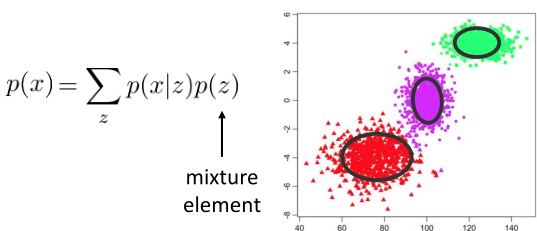
\includegraphics[width=0.5\linewidth]{figures/2020-07-01-123344_537x231_scrot.png}
	\caption{En el caso de que se tenga una distribución que por ejemplo siga una mezcla de
    gaussianas, se puede añadir una variable 'virtual' z (mixture element) que indica a que
clase pertenece cada punto.}
\label{fig:latent_gauss}
\end{figure}

También se puede dar el caso en probabilidades condicionales:
\begin{align}
    p(y|x)=\sum_z p(y|x,z)p(z)
\end{align}
Donde $p(z)$ también podría ser $p(z|x)$.

Estos modelos se vieron en Imitation Learning (el ejemplo del árbol, en el que se tiene que
elegir uno de los caminos en vez del de en medio). Normalmente una MDN como se vio en
\ref{ssub:mezclas_de_gaussianas} funciona lo suficientemente bien.

Pero puede ser que tener una variable latente que toma valores discretos no es lo
suficientemente bueno.

En el caso de que se desee aproximar distribuciones de probabilidad muy complejas,con una mezcla de
gaussianas la tarea se puede complicar. Se puede pensar que una distribución compleja viene de
una transformación no lineal de otra más sencilla, por lo que puede ser de interés coger una
distribución simple con la que se trabaje fácil como la gaussiana, aplicarle una transformación
no lineal con una red neuronal (que son aproximadores de funciones universales) y
conseguir así la distribución deseada.

La desventaja es que ahora la expresión anterior se convierte en:
\begin{align}
    p(x)=\int p(x|z)p(z)dz
\end{align}
Donde ambos términos $p(z)$ y $p(x|z)$ son sencillos (gaussiana y mezcla de gaussianas por
ejemplo), pero al ser una integral contínua de distribuciones no lineales es muy difícil de
calcular.

\begin{figure}[H]
	\centering
	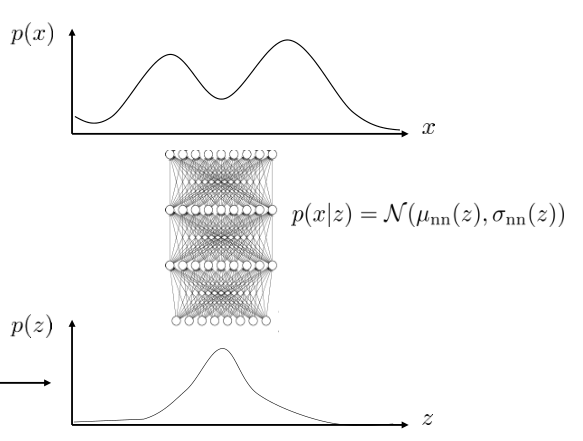
\includegraphics[width=0.5\linewidth]{figures/2020-07-01-124946_583x441_scrot.png}
\end{figure}

\subsection{Modelos con variables latentes en RL}%
\label{sub:modelos_con_variables_latentes_en_rl}

Estos modelos se usan mucho en RL.
\begin{itemize}
    \item Multi-modal Imitation Learning (el ejemplo del árbol con MDN).
    \item RL basado en modelo con imágenes. Donde el modelo de variable latente es
        $p(o_t|x_t)$. Donde se modela  $p(x_{t+1}|x_t)$ y  $p(x_t)$.
    \item Al usar RL o técnicas de control combinadas con inferencia variacional para
        modelar el comportamiento humano.
    \item En modelos generativos, donde se usa para la exploración.
\end{itemize}

\section{Inferencia variacional}%
\label{sec:inferencia_variacional}

Por ahora se trabajará con el modelo más simple: $p_\theta(x)$. Para entrenarlo se usan
los datos  $D=\{x_1,x_2,x_3,\ldots,x_N\}$. Para entrenar se usa \textit{Maximum
Likelihood}:
\begin{align}
    \theta \gets arg\max_\theta \frac{1}{N} \sum_i \log p_\theta (x_i)
\end{align}
Al tener la integral por usar variables latentes contínuas, al sustituir se tiene:
\begin{align}
    \theta \gets arg\max_\theta \frac{1}{N} \sum_i \log \left(\int p_\theta(x_i|z)p(z)dz\right)
\end{align}
Lo cual no es tratable computacionalmente.

Se podría pensar que para entrenar se puede usar \textit{expected log-likelihood}
(\textit{Expectation Maximization}). Donde se intenta estimar para cada $x$ a que $z$ pertenece,
suponer que es la correcta y actualizar según eso:
\begin{align}
\theta \leftarrow \operatorname { arg } \operatorname { max } _ { \theta } \frac { 1 } { N } \sum _ { i } E _ { z \sim p ( z | x _ { i } ) } [ \operatorname { log } p _ { \theta } ( x _ { i } , z ) ]
\end{align}
Pero se tiene que calcular $p(z|x_i)$. Cuando se tienen $z$ discretas es una tarea sencilla, pero
al ser contínua y estar estimando $p(x|z)$ mediante una red neuronal, la tarea es muy
compleja.

Por lo que se va a hacer una aproximación, en vez de calcular  $p(z|x)$, se va a aproximar
mediante una gaussiana (o otra distribución simple) $q_i=N(\mu_i,\sigma_i)$. Nótese que $q_i$ es específica para el
punto $i$ del dataset. Si se usa el objetivo de la forma correcta se puede usar $q_i$ para
delimitar la cantidad que se quiere, que es $\log p(x_i)$. Es una técnica muy sencilla,
primero se escribe el \textit{log-likelihood} que se quiere, en este caso con la integral
intratable, y se multiplica por 1, permitiendo escribir la esperanza con respecto a $q_i(z)$:
\begin{align}
    \operatorname { log } p ( x _ { i } ) &= \operatorname { log } \int _ { z } p ( x _ { i } | z
    ) p ( z )\\
                                          &=\log\int_z p(x_i|z)p(z)
                                          \frac{q_i(z)}{q_i(z)}\\
                                          &=\log E_{z\sim q_i(z)}\left[
                                          \frac{p(x_i|z)p(z)}{q_i(z)} \right]
\end{align}
Todavía se tiene la integral intratable. A continuación se va a convertir esta igualdad en una
cota usando la desigualdad de Jensen: $\log E[y]\geq E[\log y]$ (tener cuidado con los
signos).
\begin{align}
    &\geq E_{z\sim q_i(z)}\left[\log \frac{p(x_i|z)p(z)}{q_i(z)} \right]\\
    &= E _ { z \sim q _ { 1 } ( z ) } [ \operatorname { log } p ( x _ { i } | z ) + \operatorname { log } p ( z ) ] - E _ { z \sim q _ { i } ( z ) } [ \operatorname { log } q _ { i } ( z ) ]
\end{align}
El último término es simplemente la entropía de $q_i $: $H(q_i)$. Como este resultado es una
cota inferior a  $\log p(x_i)$, maximizar esta cota también maximiza $\log p(x_i)$.
Al maximizar el primer término de la expresión, lo que se está haciendo es buscar una
distribución con poca entropía en el máximo de la distribución que se está aproximando, y al
maximizar el tercer término se esta maximizando explícitamente la entropía, por lo que la
aproximación se expande por ese entorno.

 La divergencia KL se define como:
 \begin{align}
D _ { KL } ( q \| p ) = E _ { x \sim q ( x ) } [ \operatorname { log } \frac { q ( x ) } { p ( x ) } ] = E _ { x \sim q ( x ) } [ \operatorname { log } q ( x ) ] - E _ { x \sim q ( x ) } [ \operatorname { log } p ( x ) ] = - E _ { x \sim q ( x ) } [ \operatorname { log } p ( x ) ] - H ( q )
 \end{align}
sirve para saber como de diferentes son dos distribuciones. Otra forma de verlo es cuán
pequeña es la \textit{expected log probability} de una distribución sobre la otra, menos la
entropía.

Se prueba a usar la divergencia KL para aproximar $p(z|x)$.  Por simplicidad, se va a
llamar $L_i(p,q_i)$ a $E _ { x \sim q ( x ) } [ \operatorname { log } \frac { q ( x ) } { p ( x )
} ] = E _ { x \sim q ( x ) } [ \operatorname { log } q ( x ) ] - E _ { x \sim q ( x ) } [
\operatorname { log } p ( x ) ] = - E _ { x \sim q ( x ) } [ \operatorname { log } p ( x ) ] - H
( q )$. Partiendo de la intuición de que $q_i(z)$ debería aproximar $p(z|x_i)$, se
compara en términos de la divergencia KL:
\begin{align}
    \label{eq:kl_apl_1}
    D_{KL}(q_i(x_i) _ { i } \| p ( z | x _ { i } ) ) &= E _ { z \sim q _ { i } ( z ) } \left[
        \operatorname { log } \frac { q _ { i } ( z ) } { p ( z | x _ { i } ) } \right] = E _ { z
    \sim q _ { i } ( z ) } \left[ \operatorname { log } \frac { q _ { i } ( z ) p ( x _ { i } ) }
    { p ( x _ { i } , z ) } \right]\\
&= - E _ { z \sim q _ { i } ( z ) } [ \operatorname { log } p ( x _ { i } | z ) + \operatorname { log } p ( z ) ] + E _ { z \sim q _ { i } ( z ) } [ \operatorname { log } q _ { i } ( z ) ] + E _ { z \sim q _ { i } ( z ) } [ \operatorname { log } p ( x _ { i } ) ]\\
    \label{eq:kl_apl_2}
&= - E _ { z \sim q _ { i } ( z ) } [ \operatorname { log } p ( x _ { i } | z ) + \operatorname {
log } p ( z ) ] - H ( q _ { i } ) + \operatorname { log } p ( x _ { i } )\\
&=-L_i(p,q_i)+\log p(x_i)
\end{align}

Por lo que, moviendo los términos:
\begin{align}
    \operatorname { log } p ( x _ { i } ) &= D _ { KL } ( q _ { i } ( x _ { i } ) \| p ( z | x _
    { i } ) ) + L _ { i } ( p , q _ { i } ) \\ \operatorname { log } p ( x _ { i } ) &\geq L _ { i } ( p , q _ { i } )
\end{align}
Cuanto menor sea la divergencia KL, mejor será la cota inferior, por lo que interesa que tienda
a 0. Resulta que minimizar la divergencia KL con respecto a $q$ es equivalente a
maximizar la cota inferior de la evidencia con respecto a $q$. Esto se puede ver porque en las
expresiones \ref{eq:kl_apl_1} y \ref{eq:kl_apl_2} se ve que para minimizar la divergencia hay
que reducir sólo los términos que son dependientes de $q$ (todos menos el último).

En resumen, maximizar $L_i(p,q_i)$ con respecto a $q_i$ minimiza la divergencia KL.

Para hacerlo, en vez de tener ML como objetivo se tiene:
\begin{align}
    \theta \gets arg\max_\theta \frac{1}{N} \sum_i L_i(p,q_i)
\end{align}
Se quiere usar SGD con minibatches ya que es lo que se usa en DL. Se explica para un minibatch de
tamaño 1 pero para tamaños más grandes simplemente se calcula la media del gradiente.
\begin{algorithm}
    \caption{Inferencia variacional}
    \ForEach{$x_i$ (o mini-batch)}{
        Calcular $\nabla_\theta L_i(p,q_i)$:\\
        $\quad$Muestrear $z\sim q_i(x_i)$ \\
           $\quad$$\nabla_\theta L_i(p,q_i)\approx\nabla_\theta L_i(p,q_i)$ \\
        $\theta\gets\theta+\alpha\nabla_\theta L_i(p,q_i)$ \\
        Actualizar $q_i$ para maximizar $L_i(p,q_i)$
    }
\end{algorithm}

¿Cómo se actualiza $q_i$ en el último paso? Supongamos que $q_i(z)=N(\mu_i,\sigma_i)$. Entonces
se podría calcular $\nabla_\mu L_i(p,q_i)$ y $\nabla_\sigma L_i(p,q_i)$ y escalar el
gradiente. Esto funciona, pero hay un problema con este procedimiento: si se usa DL, se tiene un
gran número de datapoints. Con este procedimiento el número de parámetros es
$|\theta|+(|\mu_i||\sigma_i|)\times N$, por lo que aumenta linealmente con cada nuevo
datapoint, lo cual es un problema si se tienen millones de \textit{datapoints}. 

%\begin{align}
%D _ { KL } ( q _ { i } ( x _ { i } ) \| p ( z | x _ { i } ) ) &= E _ { z \sim q _ { i } ( z ) } [
%\operatorname { log } \frac { q _ { i } ( z ) } { p ( z | x _ { i } ) } ] = E _ { z \sim q _ { i
%} ( z ) } [ \operatorname { log } \frac { q _ { i } ( z ) p ( x _ { i } ) } { p ( x _ { i } , z )
%} ]\\
%&= E _ { z \sim q _ { i } ( z ) } [ \operatorname { log } p ( x _ { i } | z ) + \operatorname { log } p ( z ) ] - H ( q _ { i } ) + \operatorname { log } p ( x _ { i } )
%\end{align}

\section{Inferencia variacional amortizada}%
\label{sec:inferencia_variacional_amortizada}

Como todos los problemas en DL, este se resuelve con otra red neuronal. En este caso, se intenta
aprender una red $q_i(z)=q(z|x_i)\approx p(z|x_i)$, en vez de aprender $\mu_i$ y $\sigma_i$. 

Por lo que ahora hay una red que va de $z \mapsto p_\theta(x|z)$ y otra que va de $x\mapsto
q_\phi(z|x) = N(\mu_\phi(x),\sigma_\phi(x))$.

De esta forma se consigue que el número de parámetros sea independiente al número de
datapoints.  Este método se llama Inferencia variacional amortizada (\textit{Amortized variational
inference}).

El objetivo sigue siendo, como antes, acotar:
\begin{align}
\operatorname { log } p ( x _ { i } ) \geq E _ { z \sim q _ { e } ( z | x _ { i } ) } [ \operatorname { log } p _ { \theta } ( x _ { i } | z ) + \operatorname { log } p ( z ) ] + H ( q _ { \phi } ( z | x _ { i } ) )
\end{align}
donde ahora se tiene $q_\phi$. 

\begin{algorithm}
    \caption{Inferencia variacional amortizada}
    \ForEach{$x_i$ (o mini-batch)}{
        Calcular $\nabla_\theta L(p_\theta(x_i|z),q_\phi(z|x_i))$:\\
        $\quad$Muestrear $z\sim q_\phi(z|x_i)$ \\
        $\quad$$\nabla_\theta L\approx\nabla_\theta\log p_\theta(x_i|z)$ \\
        $\theta\gets\theta+\alpha\nabla_\theta L$ \\
        $\phi\gets\phi+\alpha\nabla_\phi L$
    }
\end{algorithm}

Para saber calcular $\nabla_\phi L$, vamos a escribir $L_i$ y ver que términos dependen de
$\phi$:
\begin{align}
L _ { i } = E _ { z \sim q _ { \phi } ( z | x _ { i } ) } [ \operatorname { log } p _ { \theta } ( x _ { i } | z ) + \operatorname { log } p ( z ) ] + H ( q _ { \phi } ( z | x _ { i } ) )
\end{align}
Se ve que aparece en la distribución de la esperanza y en la entropía. La entropía es
sencilla, en el caso de que $q_\phi(z|x_i)$ sea una gaussiana, se mira la expresión de la
entropía para una gaussiana en internet y ya.

En cuanto a la esperanza, se puede ver que los parámetros no influyen en el interior sino en la
distribución. Se aprecia que es lo mismo que pasaba en el objetivo de Policy Gradients, donde:
\begin{align}
J ( \phi ) = E _ { z \sim q _ { \phi } ( z | x _ { i } ) } [ r ( x _ { i } , z ) ]
\end{align}
Por lo que se puede usar el mismo truco que se usaba en ese tema para entrenar la red
neuronal:
\begin{align}
J ( \phi ) \approx \frac { 1 } { M } \sum _ { j } \nabla _ { \phi } \operatorname { log } q _ { \phi } ( z _ { j } | x _ { i } ) r ( x _ { i } , z _ { j } )
\end{align}
Lo malo es que los mismos problemas de alta varianza que se veían en el tema de Policy Gradients
también ocurren aquí. Se pueden aplicar los trucos vistos en el tema 3, pero además se puede
aplicar otro más. A diferencia de Policy Gradients, aquí no hay una noción de dinámicas
desconocidas, ya que se conoce todo: los parámetros de $q_\phi$ y sus derivadas. Por lo
que se puede usar lo que se conoce como el truco de la reparametrización
(\textit{reparametrization trick}). Consiste en calcular
$z=\mu_\phi(x)+\epsilon\sigma_\phi(x)$, donde $\epsilon\sim N(0,1)$, por lo que:
\begin{align}
    J ( \phi ) &= E _ { z \sim q _ { \phi } ( z | x _ { i } ) } [ r ( x _ { i } , z ) ]\\
               &= E _ { \epsilon \sim N ( 0,1 ) } [ r ( x _ { i } , \mu _ { \phi } ( x _ { i } ) + \epsilon \sigma _ { \phi } ( x _ { i } ) ) ]
\end{align}
Y la distribución de la esperanza pasa a ser independiente de $\phi$. Ahora para calcular el
gradiente:
\begin{itemize}
    \item Se muestrean $\epsilon_1,\ldots,\epsilon_M$ de $N(0,1)$.
    \item Se calcula el gradiente: 
        $ \nabla _ { \phi } J ( \phi ) \approx \frac { 1 } { M } \sum _ { j } \nabla _ { \phi } r ( x _ { i } , \mu _ { \phi } ( x _ { i } ) + \epsilon _ { j } \sigma _ { \phi } ( x _ { i } ) ) $
\end{itemize}
Este estimador tiene tan poca varianza que normalmente es suficiente con coger solamente una
$\epsilon$.

Otra forma de ver el truco de la reparametrización. En la práctica es muy útil expresarlo
mediante la divergencia KL ya que facilita la implementación.
\begin{align}
L _ { i } &= E _ { z \sim q _ { \phi } ( z | x _ { i } ) } [ \operatorname { log } p _ { \theta } (
x _ { i } | z ) + \operatorname { log } p ( z ) ] + H ( q _ { \phi } ( z | x _ { i } ) )\\
&= E _ { z \sim q _ { \phi } ( z | x _ { i } ) } [ \operatorname { log } p _ { \theta } ( x _ { i }
| z ) ] + E _ { z \sim q _ { \phi } ( z | x _ { i } ) } [ \operatorname { log } p ( z ) ] + H ( q
_ { \phi } ( z | x _ { i } ) )\\
&\quad\quad\quad E _ { z \sim q _ { \phi } ( z | x _ { i } ) } [ \operatorname { log } p ( z ) ] + H ( q _ { \phi }
( z | x _ { i } ) )= - D _ { KL } ( q _ { \phi } ( z | x _ { i } ) \| p ( z ) )\\
&= E _ { z \sim q _ { \phi } ( z | x _ { i } ) } [ \operatorname { log } p _ { \theta } ( x _ { i }
| z ) ] - D _ { KL } ( q _ { \phi } ( z | x _ { i } ) \| p ( z ) )\\
&= E _ { \epsilon \sim N ( 0,1 ) } [ \operatorname { log } p _ { \theta } ( x _ { i } | \mu _ {
\phi } ( x _ { i } ) + \epsilon \sigma _ { \phi } ( x _ { i } ) ) ] - D _ { KL } ( q _ { \phi } (
z | x _ { i } ) \| p ( z ) )\\
&\approx \operatorname { log } p _ { \theta } ( x _ { i } | \mu _ { \phi } ( x _ { i } ) + \epsilon \sigma _ { \phi } ( x _ { i } ) ) - D _ { KL } ( q _ { \phi } ( z | x _ { i } ) \| p ( z ) )
\end{align}

Por lo que el proceso queda:
\begin{enumerate}
    \item Se mete $x_i$ en la red parametrizada por $\phi$ y se obtiene $\mu_\phi(x_i)$ y
        $\sigma_\phi(x_i)$ 
    \item Se genera $\epsilon \in N(0,1)$.
    \item Se calcula $\mu_\phi(x_i)+\epsilon_\phi(x_i)=z$
    \item Se mete $z$ como la entrada a la otra red parametrizada por $\theta$, lo que
        devuelve $p_\theta(x_i|z)$.
    \item Se recogen todos los términos necesarios (intermedios y el final) para calcular $L$ y
        calcular los gradientes y se aplica descenso por gradiente.
\end{enumerate}

\begin{figure}[htpb]
	\centering
	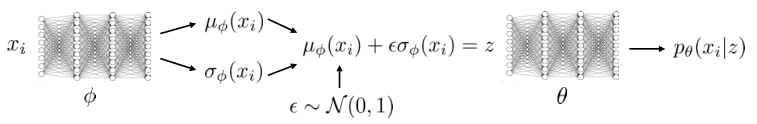
\includegraphics[width=0.8\linewidth]{figures/2020-07-01-233216_757x124_scrot.png}
	\caption{Implementación del pipeline de inferencia variacional amortizada con el truco de la reparametrización}
	\label{fig:pipeline_reparametrizacion}
\end{figure}

\subsection{Policy Gradient vs el truco de la reparametrización}%
\label{sub:policy_gradient_vs_el_truco_de_la_reparametrización}

Policy Gradients:
\begin{itemize}
    \item +: Puede manejar tanto variables latentes continuas como discretas.
    \item -: Alta varianza, lo que requiere muchas muestras y \textit{learning
        rates} pequeños.
\end{itemize}
Truco de la re parametrization:
\begin{itemize}
    \item -: Sólo se puede usar para variables latentes continuas.
    \item +: Muy sencillo de implementar.
    \item +: Varianza pequeña.
\end{itemize}

\section{Modelos generativos: autoencoder variacional}%
\label{sec:modelos_generativos_autoencoder_variacional}

Es uno de los modelos más sencillos que pueden usar el truco anterior. Es un modelo de DL. Está
formada por un encoder y un decoder. 

Para entrenarlo:
\begin{align}
\operatorname { max } _ { \theta , \phi } \frac { 1 } { N } \sum _ { j } \operatorname { log } p _ { \theta } ( x _ { i } | \mu _ { \phi } ( x _ { i } ) + \epsilon \sigma _ { \phi } ( x _ { i } ) ) - D _ { KL } ( q _ { \phi } ( z | x _ { i } ) \| p ( z ) )
\end{align}
Ejemplo de implementación: \href{https://github.com/noctrog/conv-vae}{https://github.com/noctrog/conv-vae}

\subsection{Modelos condicionales}%
\label{sub:modelos_condicionales}

Al principio del tema se comentaba que también están los modelos basados en $p(y|x)$. Los pasos
para calcular la cota inferior es el mismo pero todo ahora depende de $x_i$ :
\begin{align}
L _ { i } = E _ { z \sim q _ { \phi } ( z | x _ { i } , y _ { i } ) } [ \operatorname { log } p _ { \theta } ( y _ { i } | x _ { i } , z ) + \operatorname { log } p ( z | x _ { i } ) ] + H ( q _ { \phi } ( z | x _ { i } , y _ { i } ) )
\end{align}

Los modelos condicionados se usan por ejemplo en el caso de
\ref{ssub:latent_variable_models}, donde se inyecta ruido para que el modelo escoja una acción.

\begin{figure}[H]
	\centering
	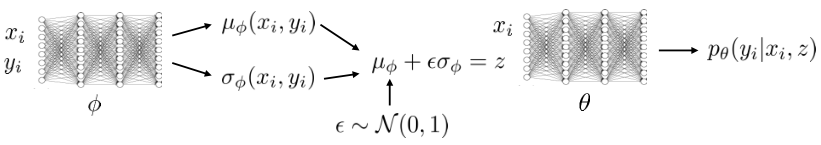
\includegraphics[width=0.8\linewidth]{figures/2020-07-01-234639_821x145_scrot.png}
	\caption{Pipeline con la distribución condicionada}
    \label{fig:pipeline_condicionado}
\end{figure}

\section{Ejemplos}%
\label{sec:ejemplos}

Publicación: Embed to Control: A Locally Linear Latent Dynamics Model for Control from Raw
Images. El modelo de esta publicación es un tipo de autoencoder variacional que tiene dinámica
en el espacio latente (no es gaussiano, tiene trayectorias). En la publicación se
visualiza la topología de $z$.

Publicación: SOLAR: Deep Structured Latent Representations for Model-Based Reinforcement
Learning. El modelo es un poco más complejo pero también funciona con autoencoders para
controlar un robot.

También se puede usar para realizar exploración y modelar el comportamiento humano.
